\chapter{Planificación}

\section{Introducción}
En este capítulo se describirá la planificación para el desarrollo del proyecto, la cual va a servir para poder
realizar un control de los avances del producto y asegurar que se cumplan los objetivos marcados en cada sprint/iteración.
Para ello, se utilizarán ciertos elementos de la metodología SCRUM, el cual definiremos brevemente a continuación:



\subsection*{SCRUM}
SCRUM es un marco de trabajo iterativo e incremental que se utiliza para desarrollar proyectos de software.
Este marco de trabajo se basa en la idea de que el desarrollo de software es un proceso complejo que se adapta continuamente
a las circunstancias. Por ello, se divide en pequeñas iteraciones que se van realizando de forma incremental y utiliza una serie de elementos
para poder controlar el desarrollo del proyecto:
\begin{itemize}
    \item \textbf{Artefactos:} Son documentos que se utilizan para controlar el desarrollo del proyecto.
    \item \textbf{Reuniones: } Se realizan cuatro tipos de reuniones de forma periódica para poder controlar y seguir el progreso del proyecto.
    \item \textbf{Roles:} Representan la responsabilidad de cada persona en el proceso.
\end{itemize}

\hfill

\begin{figure}[H]
    \centering
    \centerline{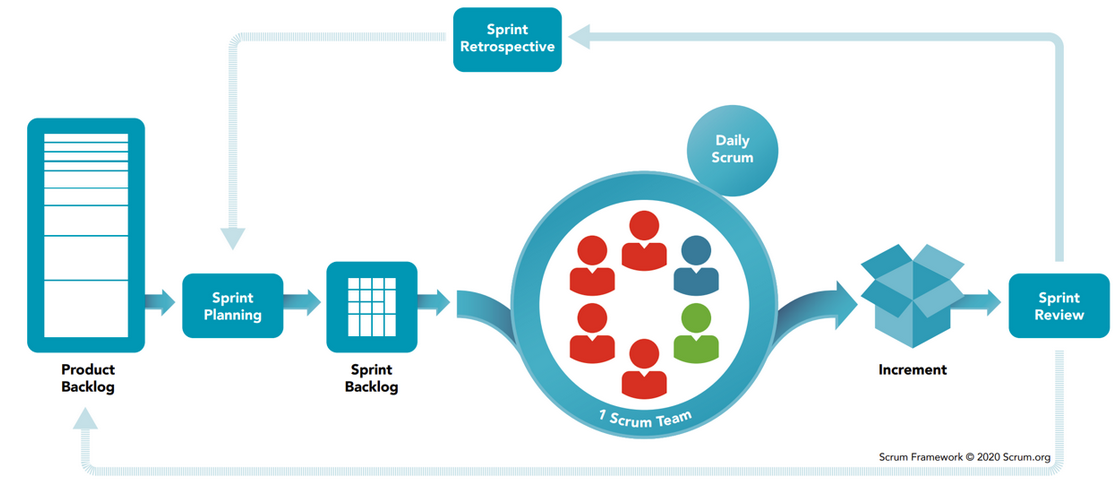
\includegraphics[width=\textwidth]{imagenes/c4/scrum.png}}
    \caption{Diagrama de la arquitectura del sistema, donde se muestra la comunicación entre el servidor y la aplicación móvil.}
    \label{fig:diagramadearquitectura}    
\end{figure}

Es importante recalcar que no voy a seguir la metodología SCRUM, sino que solo usaré algunos principios y
conceptos de metodologías ágiles debido a las condiciones en las que se va a desarrollar el proyecto
(no hay un cliente real, no hay un equipo de desarrollo real, etc.). Por tanto, se utilizarán los siguientes aspectos de SCRUM:
\begin{itemize}
    \item \textbf{Sprints:} Se definirán los Sprints (iteraciones) que se realizarán para el desarrollo del proyecto, explicando
          el objetivo de cada uno de ellos y detallando la duración y las fechas de inicio y de fin.
    \item \textbf{Historias de Usuario:} Se listarán y describirán las historias de usuario que se van a implementar en cada sprint a partir
          de los requisitos funcionales del proyecto especificados en el capítulo de Especificación de Requisitos.
    \item \textbf{Product Backlog: }Se definirá el product backlog, que es una lista de todas las funcionalidades (Historias de usuario) que se
          pretenden implementar en el proyecto. Esta lista se ordenará por prioridad de acuerdo a la importancia que tienen para el usuario final.
    \item \textbf{Velocidad:} Se calculará la velocidad de trabajo que se tendrá en el desarrollo del proyecto a partir de la cantidad de horas
          que se pretenden dedicar al proyecto cada día y la duración de los Sprints.
    \item \textbf{Puntos de historia: }Se asignarán los puntos de historia a cada historia de usuario para poder estimar la cantidad de trabajo
          que se debería realizar en cada sprint. Los valores de estos puntos de historia se calcularán a partir de la estimación de la complejidad de cada historia de usuario.
    \item \textbf{Reuniones: }Pese a no encajar exactamente en ninguna de las reuniones que hay en SCRUM, se realizarán reuniones cada dos semanas para
          poder controlar el progreso del proyecto y realizar un seguimiento de los avances. En estas reuniones se tratará:
            \begin{itemize}
                \item \textbf{Qué se ha hecho:} Se comentará el trabajo realizado desde la anterior reunión para comentar las posibles mejoras.
                \item \textbf{Qué falta por hacer: }Se comparará la planificación realizada para el Sprint con el trabajo realizado, comprobando qué cosas han podido faltar.
                \item \textbf{Qué se piensa hacer: }Se volverá a planificar si es necesario y se determinará qué trabajo se planea realizar durante el nuevo Sprint.
            \end{itemize}
\end{itemize}



\section{Velocidad}
A continuación vamos a estimar la velocidad inicial de trabajo que se tendrá en el desarrollo. Esta será una aproximación
que nos ayudará a estimar la cantidad de trabajo que se debería realizar en cada iteración. Sin embargo, esta podrá variar
y ajustarse a lo largo del proyecto en función de la cantidad de trabajo que se logre completar en cada sprint.

Para calcular la velocidad, vamos a considerar las horas de trabajo que se pretenden dedicar al proyecto cada día y tratar
de estimar cuanta cantidad de trabajo se podría realizar.

\begin{itemize}
    \item Partimos de un ``equipo de desarrollo'' de 1 miembro.
    \item Se pretende dedicar 5 horas al día de trabajo aproximadamente.
    \item Cada Sprint dura 2 semanas (14 días). Si cada día trabajamos 5 horas de forma aproximada, obtenemos un total de 70 horas
          en cada Sprint.
    \item En mi entorno, se estima que 1 PH son dos días de trabajo ideal (es decir, 10 horas).
          Esto significa que cada dos jornadas de trabajo real, se debería completar 1 PH. Sin embargo, en la realidad, esto no siempre
          es así ya que estamos realizando una aproximación.
    \item Si multiplicamos un programador por las 70 horas de trabajo y lo dividimos por el número de horas de trabajo por cada punto de historia
          (10 horas), obtenemos que deberíamos completar \textbf{7 PH} por sprint aproximadamente.
\end{itemize}

\textit{Nota: La duración de los Sprints puede variar en función de factores externos al proyecto. Pero se tratará de que duren
    2 semanas para seguir un ritmo de trabajo constante.}
    
\textit{Nota 2: Puesto que estamos realizando estimaciones y suposiciones para la planificación, esta está sujeta a cambios a
    lo largo del proyecto.}

\section{Product Backlog}
A continuación, se listarán todas las historias de usuario ordenadas por prioridad de acuerdo a la importancia que tienen para el usuario final del producto.
\begin{itemize}
    \item \textbf{HU1 - } Como usuario quiero registrarme en la aplicación para poder comenzar a utilizar sus funcionalidades. (Prioridad: Alta | Puntos de Historia: 2)
    \item \textbf{HU2 - } Como usuario quiero iniciar sesión en la aplicación para poder acceder a sus funcionalidades. (Prioridad: Alta | Puntos de Historia: 2)
    \item \textbf{HU6 - } Como usuario quiero seleccionar una lección para leer el temario. (Prioridad: Alta | Puntos de Historia: 1)
    \item \textbf{HU7 - } Como usuario quiero empezar un test de una lección. (Prioridad: Alta | Puntos de Historia: 1)
    \item \textbf{HU26 - } Como usuario quiero responder una pregunta de un test del tipo escritura de texto. (Prioridad: Alta | Puntos de Historia: 1)
    \item \textbf{HU31 - } Como usuario quiero ver todas las lecciones. (Prioridad: Alta | Puntos de Historia: 0.5)
    \item \textbf{HU8 - } Como usuario quiero responder una pregunta de un test del tipo selección múltiple. (Prioridad: Alta | Puntos de Historia: 1)
    \item \textbf{HU9 - } Como usuario quiero responder una pregunta de un test del tipo selección única. (Prioridad: Alta | Puntos de Historia: 1)
    \item \textbf{HU10 - } Como usuario quiero responder una pregunta de un test del tipo respuesta por micrófono. (Prioridad: Alta | Puntos de Historia: 8)
    \item \textbf{HU29 - } Como profesor quiero ver una lista de todas las preguntas. (Prioridad: Alta | Puntos de Historia: 0.5)
    \item \textbf{HU11 - } Como usuario quiero ver el resultado de un test. (Prioridad: Media | Puntos de Historia: 2)
    \item \textbf{HU13 - } Como usuario quiero ver mi progreso en las lecciones. (Prioridad: Media | Puntos de Historia: 2)
    \item \textbf{HU28 - } Como profesor quiero ver una lista de todas las lecciones. (Prioridad: Media | Puntos de Historia: 0.5)
    \item \textbf{HU14 - } Como profesor quiero crear una lección. (Prioridad: Media | Puntos de Historia: 1)
    \item \textbf{HU15 - } Como profesor quiero modificar el texto de una lección. (Prioridad: Media | Puntos de Historia: 2)
    \item \textbf{HU16 - } Como profesor quiero añadir contenido multimedia a una lección. (Prioridad: Media | Puntos de Historia: 2)
    \item \textbf{HU17 - } Como profesor quiero eliminar contenido multimedia de una lección. (Prioridad: Media | Puntos de Historia: 1)
    \item \textbf{HU27 - } Como profesor quiero añadir preguntas a un test del tipo entrada de texto. (Prioridad: Media | Puntos de Historia: 1)
    \item \textbf{HU18 - } Como profesor quiero añadir preguntas a un test del tipo selección múltiple. (Prioridad: Media | Puntos de Historia: 1)
    \item \textbf{HU19 - } Como profesor quiero añadir preguntas a un test del tipo selección única. (Prioridad: Media | Puntos de Historia: 1)
    \item \textbf{HU20 - } Como profesor quiero añadir preguntas a un test del tipo respuesta por micrófono. (Prioridad: Media | Puntos de Historia: 2)
    \item \textbf{HU21 - } Como profesor quiero eliminar preguntas de un test. (Prioridad: Media | Puntos de Historia: 0.5)
    \item \textbf{HU22 - } Como profesor quiero modificar preguntas de un test. (Prioridad: Media | Puntos de Historia: 1)
    \item \textbf{HU30 - } Como administrador quiero ver una lista de todos los usuarios. (Prioridad: Media | Puntos de Historia: 0.5)
    \item \textbf{HU24 - } Como administrador quiero modificar los datos de un usuario. (Prioridad: Media | Puntos de Historia: 2)
    \item \textbf{HU25 - } Como administrador quiero eliminar un usuario. (Prioridad: Media | Puntos de Historia: 0.5)
    \item \textbf{HU3 - } Como usuario quiero ver los datos personales y los logros de mi perfil. (Prioridad: Media | Puntos de Historia: 1)
    \item \textbf{HU4 - } Como usuario quiero editar los datos de mi perfil. (Prioridad: Media | Puntos de Historia: 2)
    \item \textbf{HU23 - } Como administrador quiero crear un usuario. (Prioridad: Baja | Puntos de Historia: 1)
    \item \textbf{HU12 - } Como usuario quiero ver el ranking de usuarios. (Prioridad: Baja | Puntos de Historia: 1)
    \item \textbf{HU5 - } Como usuario quiero ver el perfil de otros usuarios.  (Prioridad: Baja | Puntos de Historia: 1)

\end{itemize}

\section{Sprints}
Nuestro proyecto se pretende desarrollar en 14 Sprints. Cada Sprint tendrá una duración de 2 semanas, y se pretenden realizar una media
de 7 puntos de historia por Sprint. A continuación se especificará el contenido de cada Sprint con las fechas de inicio y fin de cada uno de ellos.

\subsection{Sprint \#1 - Documentación inicial}
\textit{24/11/2022   -   08/12/2022}\\

En este Sprint se realizará:
\begin{itemize}

    \item Definición del proyecto y del alcance.
    \item Redactar Capítulo 1 - Introducción.
    \item Redactar Capítulo 2 - Estado del Arte.
\end{itemize}
\subsection{Sprint \#2 - Documentación de requisitos}
\textit{08/12/2022   -   12/01/2023}\\

En este Sprint se planea realizar:
\begin{itemize}
    \item Revisión de la documentación inicial y corrección de errores.
    \item Redactar Capítulo 3 - Especificación de Requisitos.
\end{itemize}

\newpage

\subsection{Sprint \#3 - Documentación de HU}
\textit{12/01/2023   -   03/02/2023}\\

En este Sprint se realizará:
\begin{itemize}
    \item Revisión de la documentación de requisitos y corrección de errores.
    \item Redactar Capítulo 4 - Planificación.
    \item Redactar Capítulo 5 - Análisis del problema.
\end{itemize}
\subsection{Sprint \#4 - Diseño y comienzo del desarrollo}
\textit{03/02/2023   -   17/02/2023}\\

En este Sprint se terminará la documentación y comenzará el desarrollo con:
\begin{itemize}
    \item Revisión de la planificación y el análisis y corrección de errores.
    \item Redactar Capítulo 6 - Diseño.
    \item Preparación del backend para el desarrollo.
          \begin{itemize}
              \item Creación de la base de datos.
              \item Creación de los modelos, rutas y controladores del servidor con NodeJS.
          \end{itemize}
    \item Preparación del frontend para el desarrollo (creación de la aplicación de Flutter).
\end{itemize}

\subsection{Sprint \#5 - Registro y login de usuarios}
\textit{17/02/2023   -   03/03/2023}\\

En este Sprint se comenzará el desarrollo de la aplicación realizando las funcionalidades iniciales del usuario
que utilizará la aplicación, tales como el registro, el login, la selección de lección, etc.
\begin{itemize}
    \item HU1 - Como usuario quiero registrarme en la aplicación.
    \item HU2 - Como usuario quiero iniciar sesión en la aplicación.
    \item HU6 - Como usuario quiero seleccionar una lección para leer el temario.
    \item HU31 - Como usuario quiero ver todas las lecciones.
    \item HU28 - Como profesor quiero ver una lista de todas las lecciones.
\end{itemize}


\subsection{Sprint \#6 - Tests y progreso}
\textit{03/03/2023   -   17/03/2023}\\

Este Sprint tendrá como objetivo el desarrollo de los tests permitiendo al usuario responder a las preguntas y ver el resultado.
Además, podrá comprobar su progreso en cada lección y en la pantalla principal que muestra todas las lecciones (desbloqueando las correspondientes en su caso).
\begin{itemize}
    \item HU7 - Como usuario quiero empezar un test de una lección.
    \item HU26 - Como usuario quiero responder una pregunta de un test del tipo escritura de texto.
    \item HU8 - Como usuario quiero responder una pregunta de un test del tipo selección múltiple.
    \item HU9 - Como usuario quiero responder una pregunta de un test del tipo selección única.
    \item HU11 - Como usuario quiero ver el resultado de un test.
    \item HU13 - Como usuario quiero ver mi progreso en las lecciones.

\end{itemize}

\subsection{Sprint \#7 - Entrada de micrófono y detección de tono}
\textit{17/03/2023   -   31/03/2023}\\

En este Sprint se realizará la funcionalidad de la entrada de micrófono y la detección de tono. Puesto que la historia de usuario es muy grande y compleja, se reservará
un Sprint entero para su desarrollo. Para desarrollar esta funcionalidad, se utilizarán librerías de Flutter que permitan la entrada de audio y trabajar con el mismo.
\begin{itemize}
    \item HU10 - Como usuario quiero responder una pregunta de un test del tipo respuesta por micrófono.
\end{itemize}

\newpage
\subsection{Sprint \#8 - Funcionalidades del profesor con lecciones}
\textit{31/03/2023   -   14/04/2023}\\

En la octava iteración se comenzarán a realizar las funcionalidades relacionadas con el profesor y la gestión de las lecciones.
Además, puede que se necesite terminar la funcionalidad de la entrada de micrófono de la iteración anterior debido a que su estimación
supera los puntos de historia de un Sprint.


\begin{itemize}
    \item HU29 - Como profesor quiero ver una lista de todas las preguntas.
    \item HU14 - Como profesor quiero crear una lección.
    \item HU15 - Como profesor quiero modificar el texto de una lección.
    \item HU16 - Como profesor quiero añadir contenido multimedia a una lección.
    \item HU17 - Como profesor quiero eliminar contenido multimedia de una lección.
\end{itemize}

\subsection{Sprint \#9 - Funcionalidades del profesor con tests}
\textit{14/04/2023   -   28/04/2023}\\

En esta iteración se realizarán las funcionalidades relacionadas con el profesor y la gestión de los tests, tales como la creación, modificación y eliminación de las preguntas
de los distintos tipos. Además, se realizará la funcionalidad de ver todos los usuarios registrados en la aplicación.


\begin{itemize}
    \item HU27 - Como profesor quiero añadir preguntas a un test del tipo escritura de texto.
    \item HU18 - Como profesor quiero añadir preguntas a un test del tipo selección múltiple.
    \item HU19 - Como profesor quiero añadir preguntas a un test del tipo selección única.
    \item HU20 - Como profesor quiero añadir preguntas a un test del tipo respuesta por micrófono.
    \item HU21 - Como profesor quiero eliminar preguntas de un test.
    \item HU22 - Como profesor quiero modificar preguntas de un test.
    \item HU30 - Como administrador quiero ver una lista de todos los usuarios.
\end{itemize}


\subsection{Sprint \#10 - Funcionalidades del administrador y ranking}
\textit{28/04/2023   -   12/05/2023}\\

En la decima iteración se pretenden implementar todas las funcionalidades que tienen que ver con la administración de los usuarios, además de
dos historias relacionadas con el perfil propio del usuario.
\begin{itemize}
    \item HU24 - Como administrador quiero modificar los datos de un usuario.
    \item HU25 - Como administrador quiero eliminar un usuario.
    \item HU3 - Como usuario quiero ver los datos personales y los logros de mi perfil.
    \item HU4 - Como usuario quiero editar los datos de mi perfil.
    \item HU23 - Como administrador quiero crear un usuario.

\end{itemize}

\subsection{Sprint \#11 - Funcionalidades poco prioritarias y valor añadido}
\textit{12/05/2023   -   26/05/2023}\\

El objetivo de este Sprint es acabar todas las historias de usuario que quedan del product backlog y cuya prioridad es baja como lo es la interacción entre los distintos usuarios de la aplicación. Además, se añadirá una funcionalidad de valor añadido
en función del tiempo disponible y de las funcionalidades que se hayan podido implementar en los Sprints anteriores.
\begin{itemize}
    \item HU5 - Como usuario quiero ver el perfil de otros usuarios.
    \item HU12 - Como usuario quiero ver el ranking de usuarios.
    \item Añadir funcionalidad de valor añadido (a definir)
\end{itemize}

\subsection{Sprint \#12 - Mejoras de código}
\textit{26/05/2023   -   09/06/2023}\\

En este Sprint se pretende realizar mejoras de código en cuanto a estilo, formato y calidad del mismo. Además, se pretende dejar terminado la redacción
del séptimo capítulo del documento.
\begin{itemize}
    \item Revisar Capítulo 7 - Implementación
    \item Realizar mejoras de código.
\end{itemize}

\subsection{Sprint \#13 - Pruebas }
\textit{09/06/2023   -   23/06/2023}\\

Este Sprint se dedicará a realizar todas las pruebas necesarias para comprobar que la aplicación funciona correctamente y que no hay errores en el código, tanto
en el frontend como en el backend. También se redactará el octavo capítulo del documento con las pruebas realizadas.

\begin{itemize}
    \item Realizar pruebas de integración.
    \item Realizar pruebas de unidad.
    \item Redactar Capítulo 8 - Pruebas.
\end{itemize}

\subsection{Sprint \#14 - Conclusión y finalización del proyecto}
\textit{23/06/2023   -   15/07/2023}\\

El último Sprint se dedicará por completo a la redacción del último capítulo del documento, en el que se recogerán las conclusiones del proyecto y se realizará una revisión
de todos los capítulos para corregir errores y mejorar la redacción. Se prepará también la presentación del proyecto para la defensa ante el tribunal.
\begin{itemize}
    \item Redactar Capítulo 9 - Conclusiones.
    \item Revisión de todo el documento y corrección de errores.
    \item Preparación de la presentación del proyecto.
\end{itemize}


\section{Diagrama de Gantt}
Por último, se muestran los diagramas de Gantt de la planificación del proyecto. 


El primero es más general y representa la división del desarrollo del producto en Sprints.
En él se puede ver la duración de cada Sprint y la proporción de estos en el tiempo total del proyecto. 

\begin{figure}[H]
    \centering
    \centerline{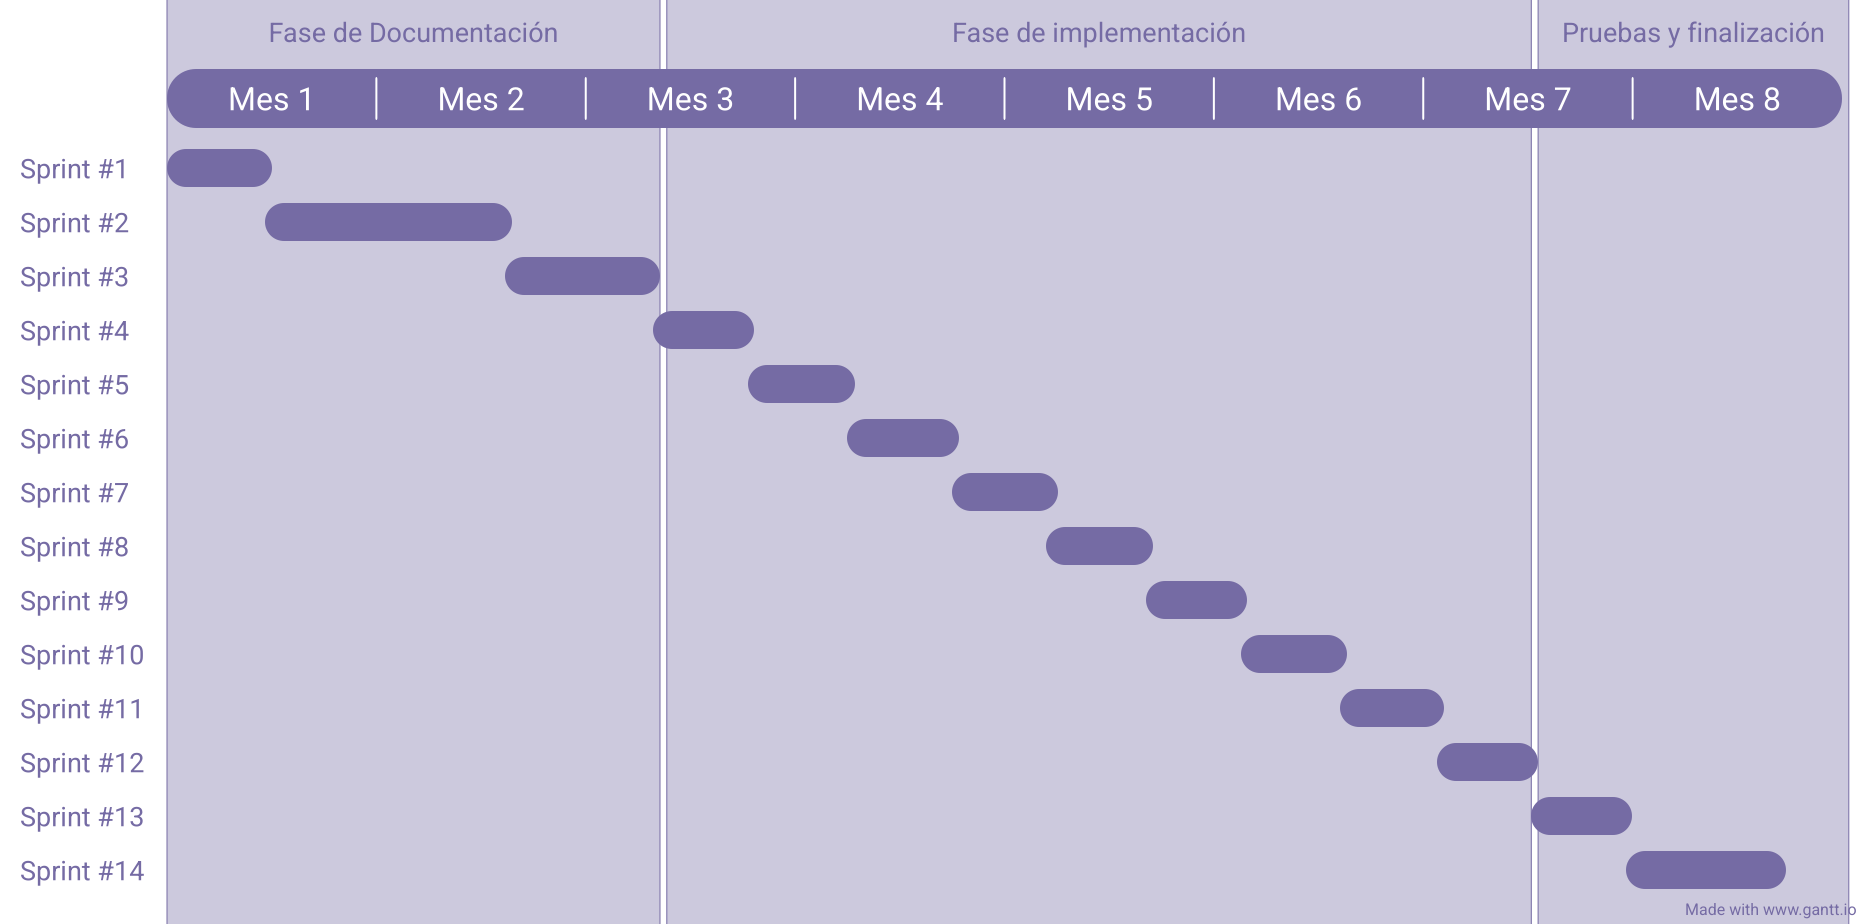
\includegraphics[width=1\textwidth]{imagenes/c4/gantt.png}}
    \caption{Diagrama de Gantt de la planificación del proyecto, divivido por Sprints.}
    \label{fig:diagrama_gantt}
\end{figure}

Como se puede ver, el proyecto se ha dividido en 14 Sprints, cada uno de ellos con una duración de dos semanas aproximadamente.
El desarrollo de cada Sprint se realizará normalmente de forma secuencial, es decir, no se empezará a desarrollar el siguiente 
Sprint hasta que no se haya terminado el anterior.
Además, es importante recalcar que los Sprints del proyecto se dividen en tres fases:
\begin{itemize}
    \item \textbf{Fase de Documentación:} en esta fase se redactará la documentación necesaria para el desarrollo del proyecto, como puede ser la especificación de requisitos, el estado del arte, la planificación, el diseño...
    A pesar de que esta sea la fase donde se redactará la mayor parte de la documentación, también se realizará esta en las fases posteriores.
    \item \textbf{Implementación:} en esta fase se desarrollará el producto, es decir, se implementarán las funcionalidades del proyecto.
    \item \textbf{Pruebas y finalización:} en esta fase se realizarán las pruebas necesarias para comprobar que el producto funciona correctamente y que no hay errores en el código. Además, se finalizará la documentación del proyecto y se preparará la presentación del mismo.
\end{itemize}


Por otro lado, a continuación se encuentra un diagrama de Gantt más detallado, en el que se puede ver la división de 
cada Sprint en historias de usuario o tareas y la duración de cada una de ellas. El diagrama se ha dividido en cuatro partes
para facilitar su visualización y su lectura, debido a la gran cantidad de información que contiene.

\begin{figure}[H]
    \centering
    \centerline{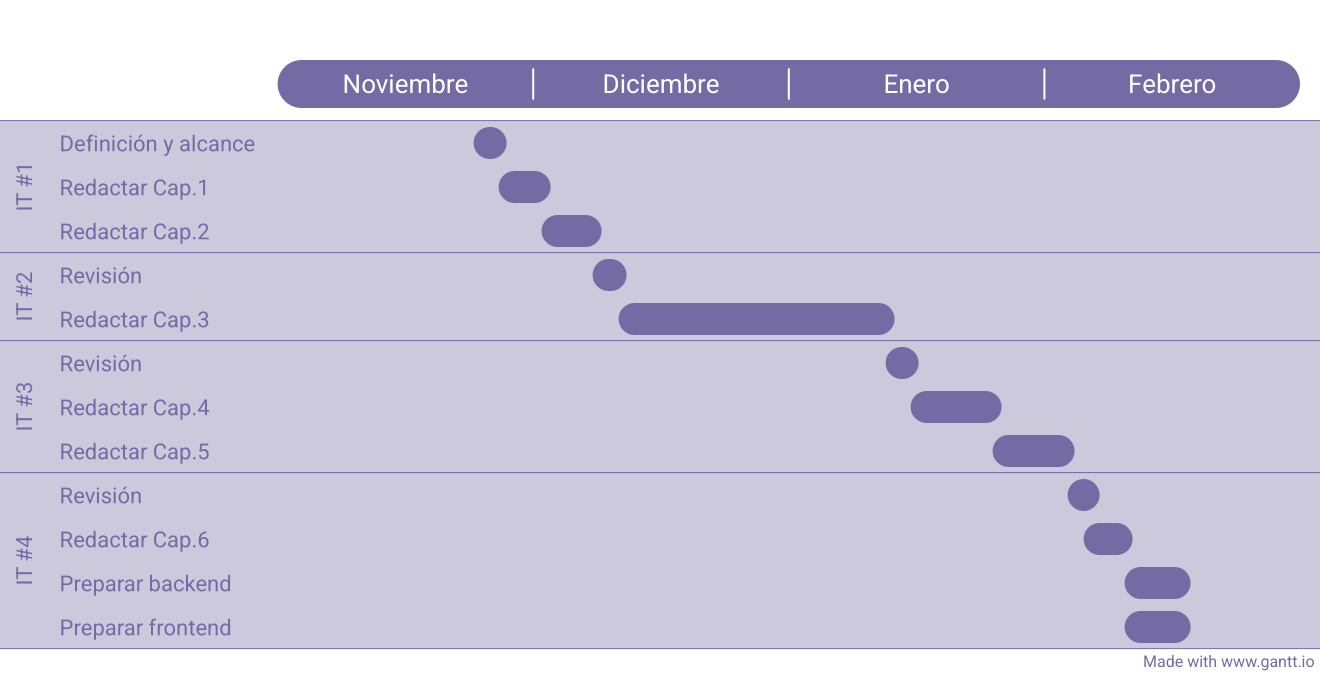
\includegraphics[width=1\textwidth]{imagenes/c4/gantt1.png}}
    \caption{Diagrama de Gantt de los cuatro primeros Sprints.}
    \label{fig:diagrama_gantt1}
\end{figure}

\begin{figure}[H]

    \centering
    \centerline{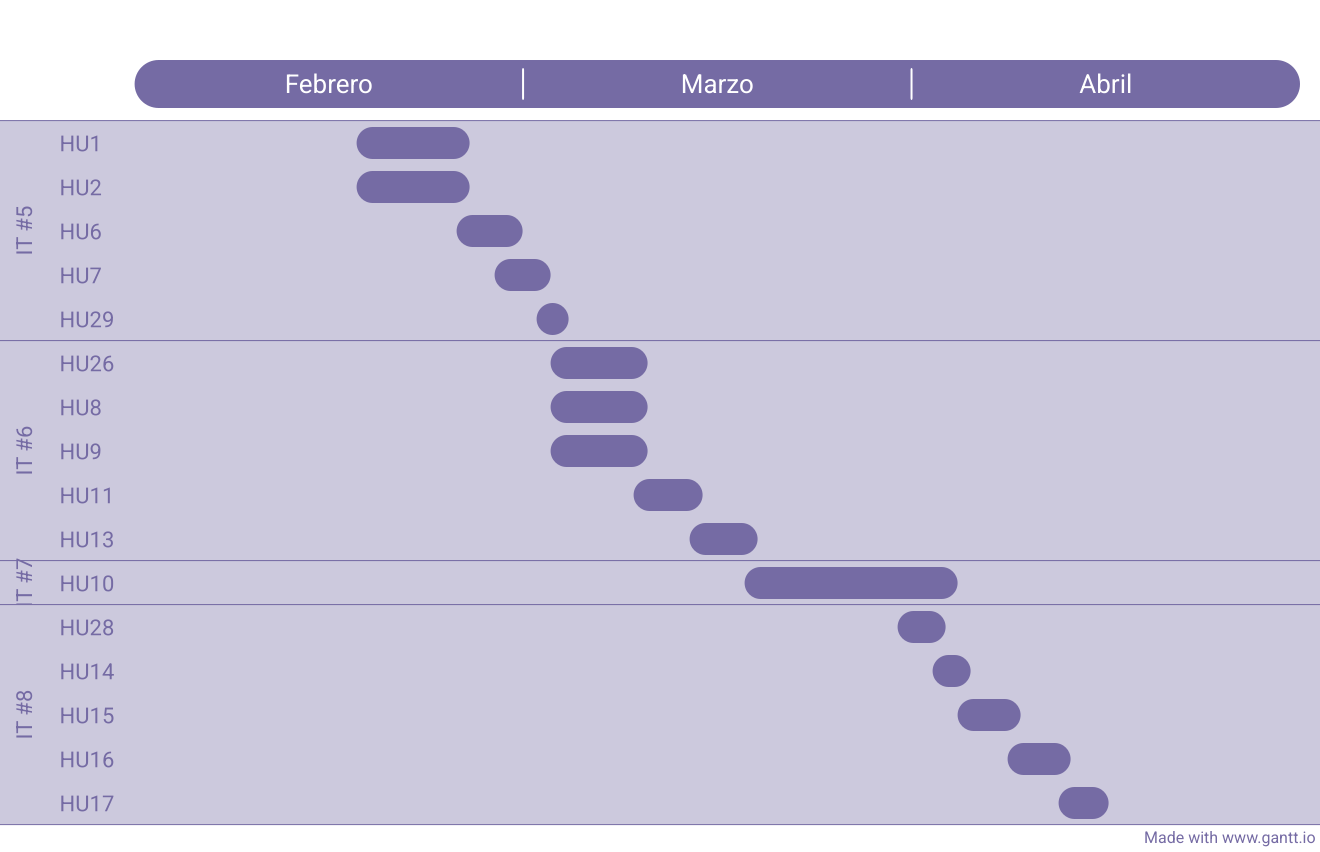
\includegraphics[width=1\textwidth]{imagenes/c4/gantt2.png}}
    \caption{Diagrama de Gantt de los Sprints 5, 6, 7 y 8.}
    \label{fig:diagrama_gantt2}
\end{figure}

\begin{figure}[H]
    \centering
    \centerline{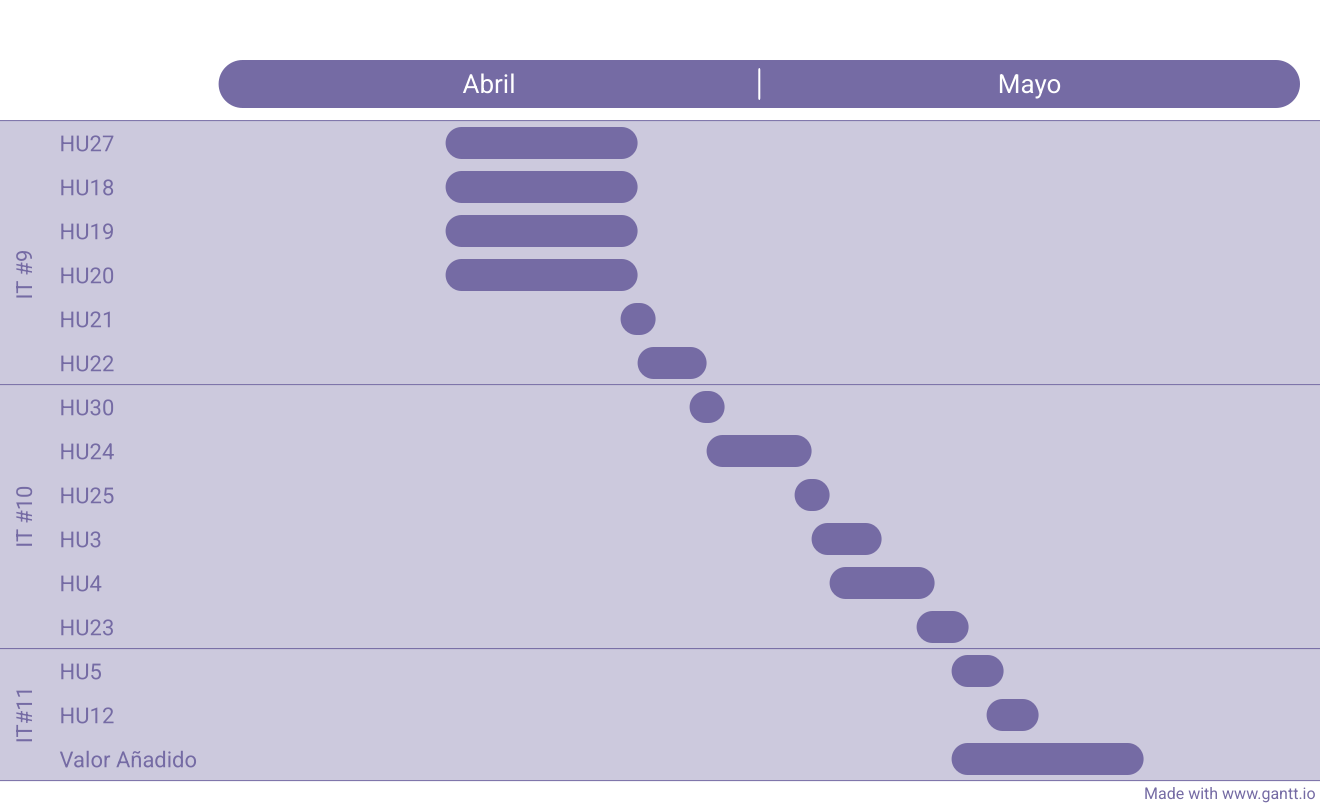
\includegraphics[width=1.1\textwidth]{imagenes/c4/gantt3.png}}
    \caption{Diagrama de Gantt de los Sprints 9, 10 y 11.}
    \label{fig:diagrama_gantt3}
\end{figure}

\begin{figure}[H]
    \centering
    \centerline{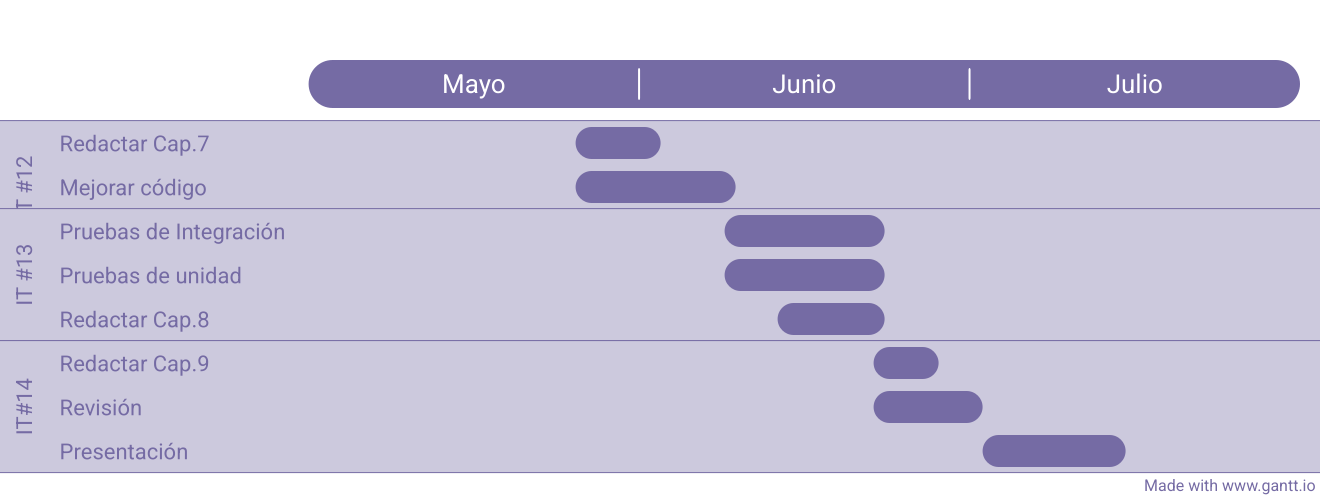
\includegraphics[width=1.2\textwidth]{imagenes/c4/gantt4.png}}
    \caption{Diagrama de Gantt de los Sprints 12, 13 y 14.}
    \label{fig:diagrama_gantt4}
\end{figure}
